\documentclass[a4paper,11pt]{article}
\usepackage{geometry} %Page setting
\usepackage{hyperref}
\usepackage{amsfonts}
\usepackage{amsmath}
\usepackage{amssymb}
%\usepackage{ctex}
\usepackage{mathtools}
\usepackage{graphicx}
\usepackage{color}

\geometry{left=2.5cm,right=2.5cm,top=2.5cm,bottom=2.5cm}  %Page setting
\makeatletter % `@' now normal "letter"
\@addtoreset{equation}{section}
\makeatother  % `@' is restored as "non-letter"
\renewcommand\theequation{\oldstylenums{\thesection}.\oldstylenums{\arabic{equation}}}
%\renewcommand\theequation{\arabic{section}.\arabic{equation}}
\renewcommand\thetable{\arabic{section}.\arabic{table}}
\renewcommand\thefigure{\arabic{section}.\arabic{figure}}


\begin{document}
\tableofcontents  %Content
\title{MAXWELL EQUATIONS}
\author{J.Guo}
\date{October 13 - November 10,2012}
\maketitle
\section{Maxwell equation}
Let $\Omega\subset\mathbb{R}^d (d=2,3)$ be an open,bounded domain with boundary $\Gamma=\partial\Omega.$
We consider the following Maxwell curl-curl problem: Find $\mathbf{u}$ such that
\begin{equation}\label{eq:cc}
\triangledown\times\triangledown\times \textbf{u} - \omega^2\mathbf{u} = \mathbf{f}, \qquad  in\ \Omega
\end{equation}
and
\begin{equation}\label{eq:cc-bc}
\mathbf{u}\times\mathbf{n} = 0. \qquad on \ \partial \Omega
\end{equation}
where $\mathbf{f}\in(L^2(\Omega))^d$ is a given vector function and $\omega\in \mathbb{R} (\omega\neq 0)$ .
$\mathbf{n}$ be the unit outward normal vector to $\Gamma$.

We also consider the following Maxwell curl-curl-grad-div problem: Find $\mathbf{u}$ such that
\begin{equation}\label{eq:ccgd}
\triangledown\times\triangledown\times \textbf{u} - \triangledown\triangledown\cdot\mathbf{u} - \omega^2\mathbf{u} = \mathbf{f}, \qquad  in\ \Omega
\end{equation}
and boundary condition: $\mathbf{u}\times\mathbf{n} = 0$ and $\triangledown\cdot\mathbf{u} = 0$.

\section{Notation}
Finite element space and $\times$-operator.
\subsection{Finite element space}
\begin{equation}\label{space:U_h}
\mathcal{U}_h = \{\mathbf{v}\in\mathbb{C}(\overline{\Omega})^d\cap H_0(\triangledown\times;\Omega): \mathbf{v}|_{T}\in(P_k(T))^d,\forall T\in\mathcal{T}_h\}
\end{equation}
\begin{equation}\label{space:U_h_+}
\mathcal{U}_{h}^{+} = \{\mathbf{v}\in\mathbb{C}(\overline{\Omega})^d\cap H_0(\triangledown\times;\Omega)\cap H(\triangledown\cdot;\Omega): \mathbf{v}|_{T}\in(P_k(T))^d,\forall T\in\mathcal{T}_h\}
\end{equation}
\begin{equation}\label{space:U_h_0}
\mathcal{U}_{h}^{0} = \{\mathbf{v}\in\mathbb{C}(\overline{\Omega})^d\cap H_0(\triangledown\times;\Omega)\cap H_0(\triangledown\cdot;\Omega): \mathbf{v}|_{T}\in(P_k(T))^d,\forall T\in\mathcal{T}_h\}
\end{equation}
where \newline\indent\indent$\mathcal{T}_h$ is a regular triangulation of $\Omega\subset\mathbb{R}^2$(tetrahedrons in $\mathbb{R}^3$),\newline
\indent\indent $h$ denotes the maximum of diameter of $T$, $\forall T\in\mathcal{T}$,\newline
\indent\indent $P_k(T)$ denotes the space of polynomials of degree $k$ on $T$,
\begin{equation}\label{space:curl}
H(\triangledown\times;\Omega) = \{\mathbf{v}\in(L^2(\Omega))^d:  \triangledown\times\mathbf{v}\in(L^2(\Omega))^{2d-3}\}
\end{equation}
\begin{eqnarray}\label{space:curl_0}
\nonumber
H_0(\triangledown\times;\Omega) & = & \{\mathbf{v}\in(L^2(\Omega))^d: \triangledown\times\mathbf{v}\in(L^2(\Omega))^{2d-3},\mathbf{v}\times\mathbf{n}|_{\partial\Omega} = 0\} \\ \nonumber
 & = & \{\mathbf{v}\in H(\triangledown\times;\Omega): \mathbf{v}\times\mathbf{n}|_{\partial\Omega} = 0\}
\end{eqnarray}

\begin{equation}\label{space:div}
H(\triangledown\cdot;\Omega) = \{\mathbf{v}\in(L^2(\Omega))^d:  \triangledown\cdot\mathbf{v}\in L^2(\Omega)\}
\end{equation}
\begin{equation}\label{space:div_0+}
\nonumber
H(\triangledown\cdot^0;\Omega) = \{\mathbf{v}\in H(\triangledown\cdot;\Omega): \triangledown\cdot\mathbf{v} = 0\}
\end{equation}
\begin{equation}\label{space:div_0}
\nonumber
H_0(\triangledown\cdot;\Omega) = \{\mathbf{v}\in H(\triangledown\cdot;\Omega): \triangledown\cdot\mathbf{v}|_{\partial\Omega} = 0\}
\end{equation}
\subsection{Curl operator}
Domain in 3D: $\mathbf{u}=(u_1,u_2,u_3)$ and $\mathbf{n} = (n_1,n_2,n_3)$, where $u_i,n_i\in\mathcal{C}^1(\Omega) (i=1,2,3)$
,$\triangledown\times\mathbf{u}$ and $\mathbf{u}\times\mathbf{n}$ are defined as follows.
\begin{displaymath}
\triangledown\times\mathbf{u} =
\left| \begin{array}{ccc}
      i & j & k \\
      \partial_x & \partial_y & \partial_z \\
       u_1 & u_2 & u_3
\end{array} \right| =
(\frac{\partial u_3}{\partial y} - \frac{\partial u_2}{\partial z},
 \frac{\partial u_1}{\partial z} - \frac{\partial u_3}{\partial x},
 \frac{\partial u_2}{\partial x} - \frac{\partial u_1}{\partial y})
\end{displaymath}
\begin{displaymath}
\mathbf{u}\times\mathbf{n} =
\left| \begin{array}{ccc}
      i & j & k \\
      u_1 & u_2 & u_3 \\
      n_1 & n_2 & n_3
\end{array} \right| = ( u_{2}n_{3} - u_{3}n_{2},u_{3}n_{1} - u_{1}n_{3},u_{1}n_{2} - u_{2}n_{1})
\end{displaymath}
Domain in 2D: $\mathbf{u}=(u_1,u_2)$ and $\mathbf{n} = (n_1,n_2)$, where $u_i,n_i,\phi\in\mathcal{C}^1(\Omega) (i=1,2)$
,$\triangledown\times\mathbf{u}$ , $\mathbf{u}\times\mathbf{n}$ ,$\phi\times\mathbf{u}$ and $\mathbf{u}\times\phi$ are defined as follows.
\begin{displaymath}
\triangledown\times\mathbf{u} = \frac{\partial u_2}{\partial x} - \frac{\partial u_1}{\partial y},\qquad \mathbf{u}\times\mathbf{n} = u_{1}n_{2} - u_{2}n_{1}
\end{displaymath}
\begin{displaymath}
\mathbf{u}\times\phi = (u_{2}\phi ,-u_{1}\phi),\qquad \phi\times\mathbf{u} = (-u_{2}\phi ,u_{1}\phi),
\end{displaymath}

Note: $\phi\rightarrow (0,0,\phi) := \widehat{\mathbf{\phi}}$,$\mathbf{u}\rightarrow (u_1,u_2,0) := \widehat{\mathbf{u}}$\newline
\indent\indent\indent$\rightrightarrows$ $\phi\times\mathbf{u} := \widehat{\mathbf{\phi}}\times\widehat{\mathbf{u}}$ and $\mathbf{u}\times\phi := \widehat{\mathbf{u}}\times\widehat{\mathbf{\phi}}$

\section{Some theories}
\subsection{Curl-Curl Problem}
Find $\mathbf{u}\in\mathcal{U}_h$, such that
\begin{equation}\label{variform:cc}
\int_{\Omega}\triangledown\times\mathbf{u}_h\cdot\triangledown\times\mathbf{v}_h - \omega^2\int_{\Omega}\mathbf{u}_h\cdot\mathbf{v}_h = \int_{\Omega}\mathbf{f}\cdot\mathbf{v}_h   \qquad \forall \mathbf{v}_h\in\mathcal{U}_h
\end{equation}\label{formula:green_curl}
we can get variational form because of $\mathbf{u}\times\mathbf{n}|_\Gamma = \mathbf{0}$ and the following $\triangledown\times$ Green's formula holds:
\begin{equation}
\int_{\Omega}\triangledown\times\mathbf{u}\cdot\mathbf{\Phi} - \int_{\Omega} u\cdot\triangledown\times\mathbf{\Phi} = \int_{\partial\Omega} \mathbf{n}\times\mathbf{u}\cdot\mathbf{\Phi}
\end{equation}
where $\mathbf{u} = (u_1,u_2,u_3),\Phi = (\phi_1,\phi_2,\phi_3)\in H(\triangledown\times;\Omega)$,\newline
Proof of Green's formula:
\begin{eqnarray}
\nonumber
& &\int_{\Omega}\triangledown\times\mathbf{u}\cdot\mathbf{\Phi} - \int_{\Omega} \mathbf{u}\cdot\triangledown\times\mathbf{\Phi} \\ \nonumber
&=&\int_{\Omega}\phi_1(\frac{\partial u_3}{\partial y} - \frac{\partial u_2}{\partial z}) +
                \phi_2(\frac{\partial u_1}{\partial z} - \frac{\partial u_3}{\partial x}) +
                \phi_3(\frac{\partial u_2}{\partial x} - \frac{\partial u_1}{\partial y})  \\ \nonumber
& &-\int_{\Omega}u_1(\frac{\partial \phi_3}{\partial y} - \frac{\partial \phi_2}{\partial z}) +
                 u_2(\frac{\partial \phi_1}{\partial z} - \frac{\partial \phi_3}{\partial x}) +
                 u_3(\frac{\partial \phi_2}{\partial x} - \frac{\partial \phi_1}{\partial y})  \\ \nonumber
&=&\int_{\Omega}(\phi_1\frac{\partial u_3}{\partial y} + u_3\frac{\partial \phi_1}{\partial y}) -
                (\phi_1\frac{\partial u_2}{\partial z} + u_2\frac{\partial \phi_1}{\partial z}) +
                (\phi_2\frac{\partial u_1}{\partial z} + u_1\frac{\partial \phi_2}{\partial z}) \\ \nonumber
& &-\int_{\Omega}(\phi_2\frac{\partial u_3}{\partial x} + u_3\frac{\partial \phi_2}{\partial x}) +
                 (\phi_3\frac{\partial u_2}{\partial x} + u_2\frac{\partial \phi_3}{\partial x}) -
                 (\phi_3\frac{\partial u_1}{\partial y} + u_1\frac{\partial \phi_3}{\partial y}) \\ \nonumber
&=&\int_{\partial\Omega} \phi_1(u_3n_2 - u_2n_3) + \phi_2(u_1n_3-u_3n_1) + \phi_3(u_2n_1 - u_1n_2) \\ \nonumber
&=&\int_{\partial\Omega} \mathbf{n}\times\mathbf{u}\cdot\mathbf{\Phi}
\end{eqnarray}
Note: while in 2D,the conclusion is the same.

$\blacktriangleright$\indent$\forall \phi\in H_{0}^{1}(\Omega)$, we have $\triangledown\phi\in H_0(\triangledown\times;\Omega)$ and $ \triangledown\times\triangledown\times(\triangledown\phi) = \mathbf{0}$.

$\blacktriangleright$\textbf{Helmholtz decomposition:} $\forall \mathbf{u}\in H_0(\triangledown\times;\Omega)$, we have $\mathbf{u} = \mathring{\mathbf{u}} + \triangledown \phi$ with $\mathring{\mathbf{u}}\in H(\triangledown\cdot^0;\Omega)$ and $\phi \in H_{0}^{1}(\Omega)$.

$\blacktriangleright$\textbf{Proposition\ 3.1} Maxwell's curl-curl problem $\Leftrightarrow$ Poisson equation + Reduced curl-curl problem.

Proof. Let curl-curl problem variational form is find $\mathbf{u}\in H_0(\triangledown\times;\Omega)$ such that
\[(\triangledown\times\mathbf{u} , \triangledown\times\mathbf{v}) - \omega^{2}(\mathbf{u},\mathbf{v}) = (\mathbf{f} , \mathbf{v}),\qquad \forall\mathbf{v}\in H_0(\triangledown\times;\Omega)\]
(1). Let $\eta\in H_{0}^{1}(\Omega)$, then $\mathbf{v} = \triangledown\eta\in H_0(\triangledown\times;\Omega)$, and
\begin{eqnarray}
\nonumber
(\triangledown\times\mathbf{u} , \triangledown\times(\triangledown\eta)) - \omega^{2}(\mathbf{u},\triangledown\eta)
 & = & (\mathbf{f} , \triangledown\eta) \\ \nonumber
- \omega^{2}(\mathring{\mathbf{u}} + \triangledown{\phi},\triangledown\eta) & = & (\mathbf{f} , \triangledown\eta) \\ \nonumber
\omega^{2}(\triangledown\cdot\mathring{\mathbf{u}},\eta) - \omega^{2}(\triangledown{\phi},\triangledown\eta) & = & (\mathbf{f} , \triangledown\eta) \ \textbf{\tiny{(Green's formula)}}
\end{eqnarray}
So $\phi\in H_{0}^{1}(\Omega)$ satisfies $- \omega^{2}(\triangledown{\phi},\triangledown\eta) =  (\mathbf{f},\triangledown\eta)\quad \forall\eta\in H_0^1(\Omega)$, which is the variational form of the Possion problem.\newline
(2). Let $\mathring{\mathbf{v}}\in H_0((\triangledown\times;\Omega)\cap H(\triangledown\cdot^0;\Omega)$, and
\begin{eqnarray}
\nonumber
(\triangledown\times\mathbf{u} , \triangledown\times\mathring{\mathbf{v}}) - \omega^{2}(\mathbf{u},\mathring{\mathbf{v}})
 & = & (\mathbf{f} , \mathring{\mathbf{v}}) \\ \nonumber
(\triangledown\times(\mathring{\mathbf{u}} + \triangledown{\phi}) , \triangledown\times\mathring{\mathbf{v}}) - \omega^{2}(\mathring{\mathbf{u}} + \triangledown{\phi},\mathring{\mathbf{v}})
 & = & (\mathbf{f} , \mathring{\mathbf{v}}) \\ \nonumber
(\triangledown\times\mathring{\mathbf{u}} , \triangledown\times\mathring{\mathbf{v}}) - \omega^{2}(\mathring{\mathbf{u}},\mathring{\mathbf{v}})
 & = & (\mathbf{f} , \mathring{\mathbf{v}})
\end{eqnarray}
Therefore, $\mathring{\mathbf{u}}$ satisfies the following reduced curl-curl problem:\newline \indent Find $\mathring{\mathbf{u}}\in H_0(\triangledown\times;\Omega)\cap H(\triangledown\cdot^0;\Omega)$ such that
\begin{eqnarray}\label{variform:cc_0}
(\triangledown\times\mathring{\mathbf{u}} , \triangledown\times\mathring{\mathbf{v}}) - \omega^{2}(\mathring{\mathbf{u}},\mathring{\mathbf{v}}) & = & (\mathbf{f} , \mathring{\mathbf{v}}), \\ \nonumber
 \forall\mathring{\mathbf{v}}&\in &H_0(\triangledown\times;\Omega) \cap  H(\triangledown\cdot^0;\Omega)
\end{eqnarray}
$\blacktriangleright$\textbf{Proposition\ 3.2} Given a Maxwell's curl-curl problem, we can get a corresponding Maxwell's curl-curl-grad-div problem.

Proof. Apply $\triangledown\cdot$ to both sides of $\triangledown\times\triangledown\times\mathbf{u} - \omega^2\mathbf{u} = \mathbf{f}$, we have $\triangledown\cdot\mathbf{u} = -\frac{1}{\omega^2}\triangledown\cdot\mathbf{f}$, then $\mathbf{u}$ satisfies the following CCGD problem:
 Find $\mathbf{u}\in H_0(\triangledown\times;\Omega)$, such that
\begin{equation}\label{eq:cc-ccgd}
\left\{\begin{array}{cc}
\triangledown\times\triangledown\times\mathbf{u} - \triangledown\triangledown\cdot\mathbf{u} - \omega^2\mathbf{u} = \mathbf{f} +  \frac{1}{\omega^2}\triangledown\triangledown\cdot\mathbf{f}&  in\ \Omega \\
\mathbf{u}\times\mathbf{n} = \mathbf{0}  & on\ \partial\Omega
\end{array}\right.
\end{equation}
In order to to get CCGD variational form \ref{eq:ccgd-form}, which will introduce in next  section, we need another boundary condition
\begin{equation}\label{eq:cc-ccgd-bc}
\triangledown\cdot\mathbf{u} = 0, \qquad on\ \partial\Omega
\end{equation}
and now $\mathbf{u}\in H_0(\triangledown\times;\Omega)\cap H_0(\triangledown\cdot;\Omega)$.
\subsection{Curl-Curl-Grad-Div problem}
The Maxwell Curl-Curl-Grad-Div(CCGD)  problem \ref{eq:ccgd} finite element variational form: Find $\mathbf{u}\in\mathcal{U}_h^{0}$, such that
\begin{equation}\label{eq:ccgd-form}
\nonumber
\int_{\Omega}\triangledown\times\mathbf{u}_h\cdot\triangledown\times\mathbf{v}_h + \
\int_{\Omega}\triangledown\cdot\mathbf{u}_h\triangledown\cdot\mathbf{v}_h - \
 \omega^2\int_{\Omega}\mathbf{u}_h\cdot\mathbf{v}_h = \
\int_{\Omega}\mathbf{f}\cdot\mathbf{v}_h   \qquad \forall \mathbf{v}_h\in\mathcal{U}_h^{0}
\end{equation}
\begin{equation}\label{variform:ccgd}
(\triangledown\times\mathbf{u}_h , \triangledown\times\mathbf{v}_h) + \
(\triangledown\cdot\mathbf{u}_h , \triangledown\cdot\mathbf{v}_h) - \
\omega^2(\mathbf{u}_h,\mathbf{v}_h) = (\mathbf{f},\mathbf{v}_h)  \qquad \forall \mathbf{v}_h\in\mathcal{U}_h^{0}
\end{equation}

$\blacktriangleright$ $\triangledown\cdot$ Green's formula: $\int_{\Omega}\mathbf{v}\cdot\triangledown\phi + \int_{\Omega}\triangledown\cdot\mathbf{v}\phi = \
\int_{\partial\Omega}\phi\mathbf{v}\cdot\mathbf{n}$

$\blacktriangleright$ When $\triangledown\cdot\mathbf{f} = 0$, the solution $\mathbf{u}$ of CCDG, if exists, belongs to
the space $H(\triangledown\cdot^0;\Omega)$, then CCDG $\Leftrightarrow$ CC.

$\blacktriangleright$ [\textbf{Fredholm Theory}]The CCGD problem is well-posed as long as $\omega^2\neq\lambda_{i}$, where $0\leq\lambda_{1}\leq\lambda_{2}\leq\cdots\rightarrow\infty$ are eigenvalues defined by the following eigen-problem:
\begin{equation}
\nonumber
(\triangledown\times\mathbf{u} , \triangledown\times\mathbf{v}) - \
(\triangledown\cdot\mathbf{u} , \triangledown\cdot\mathbf{v}) = \
\lambda_i(\mathbf{u}_h,\mathbf{v})
\end{equation}
\[\nonumber\qquad\qquad\qquad\qquad\qquad\qquad\qquad \forall \mathbf{v}\in H_0(\triangledown\times;\Omega)\cap H(\triangledown\cdot;\Omega)\]

$\blacktriangleright$ [\textbf{Regularity}]The regularity of the solution of CCGD problem is closely related to the regularity of the
Laplace operator with homogeneous Dirichlet or Neumann boundary conditions.

Proof. For simplicity, we assume $\Omega$ is simply connected.
\newline If $\mathbf{u}\in H_0(\triangledown\times;\Omega)\cap H(\triangledown\cdot;\Omega)$, there is an unique Helmholtz decomposition \[\mathbf{u} = \mathring{\mathbf{u}} + \triangledown{\phi}\]

where $\mathring{\mathbf{u}}\in H_0(\triangledown\times;\Omega)\cap H(\triangledown\cdot^0;\Omega)$ and $\phi\in H_{0}^{1}(\Omega)$
\begin{center}
$\begin{array}{ccc}
\triangledown\cdot\mathring{\mathbf{u}} = 0 & \Rightarrow & \exists\psi\in H^1(\Omega), s.t.\ \mathring{\mathbf{u}} = \triangledown\times\psi \\
& \Rightarrow & \mathbf{u} = \triangledown\times\psi + \triangledown\phi
\end{array}$
\end{center}

(1). Apply $\triangledown\cdot$ to both sides of $\mathbf{u} = \triangledown\times\psi + \triangledown\phi$, we have
\[\triangledown\cdot\mathbf{u} = \triangledown\cdot(\triangledown\times\psi) + \triangledown\cdot(\triangledown\phi) = \triangle\phi\]
So the function $\phi\in H_0^1(\Omega)$ satisfies the following Dirichlet boundary value problem:
\begin{equation}\label{eq:Dirichlet}
\left\{\begin{array}{cc}
\triangle\phi = \triangledown\cdot\mathbf{u} &  in\ \Omega \\
\phi = 0  & on\ \partial\Omega
\end{array}\right.
\end{equation}

(2). Apply $\triangledown\times$ to both sides of $\mathbf{u} = \triangledown\times\psi + \triangledown\phi$, we have
\[\triangledown\times\mathbf{u} = \triangledown\times(\triangledown\times\psi) + \triangledown\times(\triangledown\phi) = -\triangle\psi\]
[since $\triangle\omega = - \triangledown\times\triangledown\times\omega$,
$\triangle\mathbf{w} = - \triangledown\times\triangledown\times\mathbf{w} + \triangledown\triangledown\cdot\mathbf{w}$]\newline
So the function $\psi\in H^1(\Omega)$ satisfies the following Neumann boundary value problem:
\begin{equation}\label{eq:Neumann}
\left\{\begin{array}{cc}
\triangle\psi = - \triangledown\times\mathbf{u} &  in\ \Omega \\
\frac{\partial\psi}{\partial\mathbf{n}} = 0  & on\ \partial\Omega
\end{array}\right.
\end{equation}
[since on $\partial\Omega$ $0 = \mathring{\mathbf{u}}\times\mathbf{n} = (\triangledown\times\psi)\times\mathbf{n} = -\frac{\partial\psi}{\partial\mathbf{n}}$]

Since $\mathbf{u} = \triangledown\times\psi + \triangledown\phi$, the regularity of $\mathbf{u}$ can be derived through the elliptic
regularity theory on polygonal domains. (P.Grisvard. 1985.)

\newpage
\section{Numerical experiments}
\subsection{Structure numerical solution}
\textbf{Step 1:} find $\mathbf{u}\in H(\triangledown\times;\Omega)$, such that $\mathbf{u}\times\mathbf{n}|_{\partial\Omega} = \mathbf{0}$;\newline
\indent\indent (e.g. find $\phi|_{\partial\Omega} = 0$, let $\mathbf{u} = \triangledown\phi$, then $\mathbf{f} = -\omega^2\triangledown\phi$)
\newline\textbf{Step 2:} find $\mathbf{u}^{*}$ depend on $\mathbf{u}$,such that $\triangledown\cdot\mathbf{f}^* = \mathbf{0}$.\newline
\indent\indent (e.g. fine $\theta$, such that $-\omega^2\triangle\theta = \triangledown\cdot\mathbf{f}$ and $\theta|_{\partial\Omega} = 0$. Let $\mathbf{u}^{*} = \mathbf{u} - \triangledown{\theta}$, then $\mathbf{f}^{*} = \mathbf{f} + \omega^2\triangledown\theta$ satisfied $\triangledown\cdot\mathbf{f}^* = \mathbf{0}$)
\newline\textbf{Corollary\ 4.1}  When $\triangledown\cdot\mathbf{f} = 0$, the solution $\mathbf{u}$ of CCDG, if exists, belongs to
the space $H(\triangledown\cdot^0;\Omega)$ and CCDG Maxwell problem  $\Leftrightarrow$ CC Maxwell problem.

\subsection{Smooth solution domain}
\begin{figure}[bhpt]
  \hspace{-5.pt}
  \begin{minipage}[b]{0.5 \textwidth}
    \centering
    \includegraphics[width=2in]{Image/fig_S2D}\\
    \caption{$\Omega = [0,1]^2$.}\label{fig:fig_S2D}
  \end{minipage}
  \hspace{-0.2in}
  \begin{minipage}[b]{0.5 \textwidth}
    \centering
    \includegraphics[width=2in]{Image/fig_S3D}
    \caption{$\Omega = [0,1]^3$.}\label{fig:fig_S3D}
  \end{minipage}
\end{figure}

\subsection{Non-smooth solution domain}

\begin{figure}[bhpt]
  \hspace{-5.pt}
  \begin{minipage}[b]{0.5 \textwidth}
    \centering
    \includegraphics[width=2in]{Image/fig_N2D}\\
    \caption{$\Omega = [-1,1]^2/[0,1]\times[-1,0]$.}\label{fig:fig_N2D}
  \end{minipage}
  \hspace{-0.2in}
  \begin{minipage}[b]{0.5 \textwidth}
    \centering
    \includegraphics[width=2in]{Image/fig_N3D}\\
    \caption{$\Omega = [-1,1]^3/[0,1]^3$}\label{fig:fig_N3D}
  \end{minipage}
\end{figure}
\newpage
\subsection{Exact Solution}
Put $\omega = 1$, The exact solution of Figure\ref{fig:fig_S2D} and Figure\ref{fig:fig_N2D} as following

\textbf{S2DI} Let $p(x,y) = e^{x + y}\sin(\pi x)\sin(\pi y)$, we defined exact solution $\mathbf{u} = \triangledown \big(p(x,y)\big)$
\begin{equation}
\mathbf{u} = \
\left( \begin{array}{c}
      u_1 \\
      u_2 \\
\end{array} \right) =
\left( \begin{array}{c}
      e^{x+y}\sin(\pi y)(\sin(\pi x) + \pi\sin(\pi x)) \\
      e^{x+y}\sin(\pi x)(\sin(\pi y) + \pi\sin(\pi y))
\end{array} \right)
\end{equation}
\indent\indent\indent\indent\indent\indent\indent\indent$\mathbf{u}\in H_0(\triangledown\times;\Omega)$, $\triangledown\cdot\mathbf{u}|_{\partial\Omega} \neq 0$

\indent\indent\indent\indent\indent\indent\indent\indent$\mathbf{f} = -\mathbf{u}.$

\textbf{S2DII} CC problem (\ref{eq:cc} and \ref{eq:cc-bc}) CCGD variational form(\ref{eq:cc-ccgd} and \ref{eq:cc-ccgd-bc}).
\begin{equation}
\mathbf{u} =
\left( \begin{array}{c}
      u_1 \\
      u_2 \\
\end{array} \right) =
\left( \begin{array}{c}
      e^{y}y(y-1) \\
      e^{x}sin(\pi x) \\
\end{array} \right)
\end{equation}

\indent\indent\indent\indent\indent\indent\indent\indent$\mathbf{u}\in H_0(\triangledown\times;\Omega)\cap H_0(\triangledown\cdot;\Omega)$,
\begin{equation}
\mathbf{f} =  \triangledown\times\triangledown\times\mathbf{u}  -\mathbf{u}=
\left( \begin{array}{c}
      -2 e^{y}y(y+1) \\
      e^{x}\big((\pi^2 -2)\sin(\pi x) - 2 \pi \cos(\pi x)\big) \\
\end{array} \right)
\end{equation}

\textbf{N2DI}  Let $\psi = r^{\frac{2}{3}}\sin(\frac{2}{3}\theta)\phi(r)$, where $(r,\theta)$ are the polar coordinates at the origin and the cut-off function $\varphi(r)$ is given by
\begin{equation}
\nonumber
\phi(r) = \left\{\begin{array}{cc}
1,  &  r\leq 0.25 \\
-16(r - 0.75)^3[5 + 15(r - 0.75) + 12(r - 0.75)^2], & 0.25\leq r\leq 0.75\\
0,  &  r\geq 0.75
\end{array}\right.
\end{equation}

The exact solution is chosen to be  $\mathbf{u} = \triangledown\times\psi = (u_1 , u_2)'$, then we have
\begin{equation}
\left( \begin{array}{c}
      u_1 \\
      u_2 \\
\end{array} \right) =
\left( \begin{array}{c}
      \frac{2}{3}r^{\frac{2}{3}}\sin(\frac{1}{3}\theta)\phi(r) + r^{\frac{5}{3}}\cos(\frac{2}{3}\theta)\sin(\theta)\varphi^{'}(r) \\
      - \frac{2}{3}r^{\frac{2}{3}}\cos(\frac{1}{3}\theta)\phi(r) - r^{\frac{5}{3}}\cos(\frac{2}{3}\theta)\cos(\theta)\varphi^{'}(r)  \\
\end{array} \right)
\end{equation}
\indent\indent\indent\indent\indent\indent\indent\indent$\mathbf{u}\in H_0(\triangledown\times;\Omega)\cap H_0(\triangledown\cdot;\Omega)$,
\begin{equation}
\nonumber
\mathbf{f} = -\mathbf{u} - \triangledown\times\triangledown\times\mathbf{u}
\end{equation}

\textbf{N2DII} Similar to N2DI let $\varphi = r^{\frac{2}{3}}\sin(\frac{2}{3}\theta)(x^2 - 1)(y^2 - 1)$, the exact solution is given by
\begin{equation}
\mathbf{u} = \triangledown\varphi = \left(\begin{array}{c}
-\frac{2}{3}r^{\frac{2}{3}}\sin(\frac{1}{3}\theta)(x^2 - 1)(y^2 - 1) + 2x r^{\frac{2}{3}}\sin(\frac{2}{3}\theta)(y^2 - 1) \\
\frac{2}{3}r^{\frac{2}{3}}\cos(\frac{1}{3}\theta)(x^2 - 1)(y^2 - 1) + 2y r^{\frac{2}{3}}\sin(\frac{2}{3}\theta)(x^2 - 1)
\end{array}\right)
\end{equation}
\indent\indent\indent\indent\indent\indent\indent\indent$\mathbf{u}\in H_0(\triangledown\times;\Omega)$,$\triangledown\cdot\mathbf{u}|_{\partial\Omega} \neq 0$

\indent\indent\indent\indent\indent\indent\indent\indent$\mathbf{f} = -\mathbf{u} - \triangledown\triangledown\cdot\mathbf{u}.$

\textbf{S3D}

\textbf{N3D}

\textbf{Remark:} In order to get the correct error rate, we give the following remarks:

1.while $\triangledown\cdot\mathbf{u}|_{\Omega}=\mathbf{0}$, we consider ccgd problem(eq \ref{eq:cc-ccgd} and eq \ref{eq:cc-ccgd-bc}),instead of cc problem(eq \ref{eq:cc} and eq \ref{eq:cc-bc}). Variational form is eq \ref{variform:ccgd}.

2.while $\triangledown\cdot\mathbf{u}|_{\Omega}\neq\mathbf{0}$, it is necessary to add $\triangledown\cdot\mathbf{u} = g\ (in\ \Omega )$ to cc problem(eq \ref{eq:cc} and eq \ref{eq:cc-bc}), and finite element variational form is: Find $\mathbf{u}_h\in U_{h}^{+}$ such that
\begin{equation}\label{eq:cc_div_neq_0}
(\triangledown\times\mathbf{u}_h,\triangledown\times\mathbf{v}_h) + \
(\triangledown\cdot\mathbf{u}_h,\triangledown\cdot\mathbf{v}_h) -\
\omega^2(\mathbf{u}_h,\mathbf{v}_h) = \
(f,\mathbf{v}_h) + (g,\triangledown\cdot\mathbf{v}_h),\ \forall\mathbf{v}_h\in U_{h}^{+}
\end{equation}
\subsection{Error}
\begin{center}
Table 4.1: {Relative error in $L^2$-norm for curl-curl $P_1$ approximation}
\begin{tabular}{|c|c|c|c|c|c|c|}
  \hline
  \multicolumn{1}{|c}{$\|\mathbf{u} - \mathbf{u}_{h}\|_{0}$} & \multicolumn{2}{|c}{S2DI} & \multicolumn{2}{|c}{S2DII}& \multicolumn{2}{|c|}{N2D} \\
  \hline
    Mesh  & u1 Error & Ratio & u1 Error & Ratio & Error & Ratio  \\
  \hline
    1/8    &  7.297e-02  &        &  2.359e-02  &	    & 0.589423  &       \\
    1/16   &  1.886e-02  &  3.87  &  5.943e-03  & 3.97  & 0.635463  &       \\
    1/32   &  4.754e-03  &  3.97  &  1.489e-03  & 3.99  & 0.655565  &       \\
    1/64   &  1.191e-03  &  3.99  &  3.723e-04  & 4.00  & 0.665602  &       \\
    1/128  &  2.979e-04  &  4.00  &  9.310e-05  & 4.00  &           &       \\
    1/256  &  7.448e-05  &  4.00  &  2.328e-05  & 4.00  &           &       \\
  \hline
\end{tabular}
\end{center}
\begin{center}
Table 4.2: {Relative error in $\triangledown\times L^2$-norm for curl-curl $P_1$ approximation}
\begin{tabular}{|c|c|c|c|c|c|c|}
  \hline
  \multicolumn{7}{|c|}{ $\|\triangledown\times(\mathbf{u} - \mathbf{u}_h)\|_0 + \|\triangledown\cdot(\mathbf{u} - \mathbf{u}_h)\|_0$}  \\
  \hline
  \multicolumn{1}{|c}{$P_1$} & \multicolumn{2}{|c}{S2DI} & \multicolumn{2}{|c}{S2DII}& \multicolumn{2}{|c|}{N2D}   \\
  \hline
    Mesh  & u1 Error & Ratio & u1 Error & Ratio & Error & Ratio  \\
  \hline
    1/8   &  2.224e-01  &      & 1.653e-01  &	   & 0.5894231  &       \\
    1/16  &  1.116e-01  & 1.99 & 8.297e-02  & 1.99 & 0.635463   &       \\
    1/32  &  5.581e-02  & 2.00 & 4.152e-02  & 2.00 & 0.655565   &       \\
    1/64  &  2.791e-02  & 2.00 & 2.077e-02  & 2.00 & 0.665602   &       \\
    1/128 &  1.396e-02  & 2.00 & 1.038e-02  & 2.00 &            &       \\
    1/256 &  6.978e-03  & 2.00 & 5.192e-03  & 2.00 &            &       \\
  \hline
\end{tabular}
\end{center}
\begin{center}
Table 4.3: {Relative error in $L^2$-norm for curl-curl $P_2$ approximation}
\begin{tabular}{|c|c|c|c|c|c|c|}
  \hline
  \multicolumn{1}{|c}{$\|\mathbf{u} - \mathbf{u}_{h}\|_{0}$} & \multicolumn{2}{|c}{S2DI} & \multicolumn{2}{|c}{S2DII}& \multicolumn{2}{|c|}{N2D} \\
  \hline
    Mesh  & u1 Error & Ratio & u1 Error & Ratio & Error & Ratio  \\
  \hline
    1/8    & 1.414e-03 &	  &  4.419e-04 &	       		  & 0.636119  &       \\
    1/16   & 1.766e-04 & 8.01 &  5.564e-05 &  7.94 			  & 0.658902  &       \\
    1/32   & 2.2137e-05& 8.00 &  6.981e-06 &  7.97 			  & 0.670074  &       \\
    1/64   & 2.7723e-06& 7.98 &  8.732e-07 &  7.99 			  &           &       \\
    1/128  & 3.4380e-07& 8.06 &  1.021e-07 &{\color{red}8.56} &           &       \\
  \hline
\end{tabular}
\end{center}
\begin{center}
Table 4.4: {Relative error in $\triangledown\times L^2$-norm for curl-curl $P_2$ approximation}
\begin{tabular}{|c|c|c|c|c|c|c|}
  \hline
  \multicolumn{7}{|c|}{$\|\triangledown\times(\mathbf{u} - \mathbf{u}_h)\|_0 + \|\triangledown\cdot(\mathbf{u} - \mathbf{u}_h)\|_0$}  \\
  \hline
  \multicolumn{1}{|c}{$P_2$} & \multicolumn{2}{|c}{S2DI} & \multicolumn{2}{|c}{S2DII}& \multicolumn{2}{|c|}{N2D}   \\
  \hline
    Mesh  & u1 Error & Ratio & u1 Error & Ratio & Error & Ratio  \\
  \hline
    1/8   &  1.7082e-02 &       & 6.832E-03 &	   &  0.960385  &       \\
    1/16  &  4.3392e-03 &  3.94 & 1.721E-03 & 3.97 &  0.98068   &       \\
    1/32  &  1.0914e-03 &  3.98 & 4.317E-04 & 3.99 &  0.990626  &       \\
    1/64  &  2.7354e-04 &  3.99 & 1.081E-04 & 3.99 &            &       \\
    1/128 &  6.8460e-05 &  4.00 & 2.704E-05 & 4.00 &            &       \\
    1/256 &  1.7124e-05 &  4.00 &           &      &            &       \\
  \hline
\end{tabular}
\end{center}
\begin{center}
Table 4.5: {Relative error in $L^2$-norm for curl-curl $P_3$ approximation}
\begin{tabular}{|c|c|c|c|c|c|c|}
  \hline
  \multicolumn{1}{|c}{$\|\mathbf{u} - \mathbf{u}_{h}\|_{0}$} & \multicolumn{2}{|c}{S2DI} & \multicolumn{2}{|c}{S2DII}& \multicolumn{2}{|c|}{N2D}  \\
  \hline
    Mesh  & u1 Error & Ratio & u1 Error & Ratio & Error & Ratio  \\
  \hline
    1/8   &  3.615e-05 &	                & 3.335e-06 &   				&           &     \\
    1/16  &  2.260e-06 & 16.00 				& 2.043e-07	& 16.32  			&           &     \\
    1/32  &  1.411e-07 & 16.01 				& 1.288e-08	& 15.86  			&           &     \\
    1/64  &  8.807e-09 & 16.02              & 3.094e-09	& {\color{red}4.16} &           &     \\
    1/128 &  5.956e-10 & {\color{red}14.79} & 1.638e-09	& {\color{red}1.89} &           &     \\
  \hline
\end{tabular}
\end{center}
\begin{center}
Table 4.6: {Relative error in $\triangledown\times L^2$-norm for curl-curl $P_3$ approximation}
\begin{tabular}{|c|c|c|c|c|c|c|}
  \hline
  \multicolumn{7}{|c|}{$\|\triangledown\times(\mathbf{u} - \mathbf{u}_h)\|_0 + \|\triangledown\cdot(\mathbf{u} - \mathbf{u}_h)\|_0$}\\
  \hline
  \multicolumn{1}{|c}{$P_3$} & \multicolumn{2}{|c}{S2DI} & \multicolumn{2}{|c}{S2DII}& \multicolumn{2}{|c|}{N2D}  \\
  \hline
    Mesh  & u1 Error & Ratio & u1 Error & Ratio & Error & Ratio \\
  \hline
    1/8   &  5.061e-04  &	   & 1.353e-04	&	   &          &      \\
    1/16  &  6.429e-05	& 7.87 & 1.702e-05	& 7.95 &          &      \\
    1/32  &  8.086e-06	& 7.95 & 2.133e-06	& 7.98 &          &     \\
    1/64  &  1.013e-06	& 7.98 & 2.669e-07	& 7.99 &          &      \\
    1/128 &  1.267e-07	& 7.99 & 3.338e-08	& 8.00 &          &      \\
  \hline
\end{tabular}
\end{center}

\subsection{Rate}
\begin{figure}[bhpt]
  \hspace{35.pt}
  \begin{minipage}[t]{0.4 \textwidth}
    \centering
    \includegraphics[width=2.5in]{Image/Rate01}\\
    \caption{Rate of S2DI,S2DII in $\|\mathbf{u} - \mathbf{u}_h\|_0$ norm.}\label{fig:fig_Rate01}
  \end{minipage}
  \hspace{0.3in}
  \begin{minipage}[t]{0.4 \textwidth}
    \centering
    \includegraphics[width=2.5in]{Image/Rate02}\\
    \caption{Rate of S2DI,S2DII in $\|\triangledown\times(\mathbf{u} - \mathbf{u}_h)\|_0 + \|\triangledown\cdot(\mathbf{u} - \mathbf{u_h})\|_0$ norm.} \label{fig:fig_Rate02}
  \end{minipage}
\end{figure}
\begin{figure}[bhpt]
  \hspace{35.pt}
  \begin{minipage}[t]{0.4 \textwidth}
    \centering
    \includegraphics[width=2.5in]{Image/Rate1}\\
    \caption{Rate of S2DI,S2DII in $\|\mathbf{u} - \mathbf{u}_h\|_0$ norm.}\label{fig:fig_Rate1}
  \end{minipage}
  \hspace{0.3in}
  \begin{minipage}[t]{0.4 \textwidth}
    \centering
    \includegraphics[width=2.5in]{Image/Rate2}\\
    \caption{Rate of S2DI,S2DII in $\|\triangledown\times(\mathbf{u} - \mathbf{u}_h)\|_0 + \|\triangledown\cdot(\mathbf{u} - \mathbf{u_h})\|_0$ norm.} \label{fig:fig_Rate2}
  \end{minipage}
\end{figure}
\begin{figure}[bhpt]
  \hspace{35.pt}
  \begin{minipage}[t]{0.4 \textwidth}
    \centering
    \includegraphics[width=2.5in]{Image/Rate3}\\
    \caption{Rate of S2DI,S2DII in $\|\mathbf{u} - \mathbf{u}_h\|_0$ norm.}\label{fig:fig_Rate3}
  \end{minipage}
  \hspace{0.3in}
  \begin{minipage}[t]{0.4 \textwidth}
    \centering
    \includegraphics[width=2.5in]{Image/Rate4}\\
    \caption{Rate of S2DI,S2DII in $\|\triangledown\times(\mathbf{u} - \mathbf{u}_h)\|_0 + \|\triangledown\cdot(\mathbf{u} - \mathbf{u_h})\|_0$.} \label{fig:fig_Rate4}
  \end{minipage}
\end{figure}

\newpage
\subsection{Figure}

\begin{figure}[bhpt]
  \hspace{35.pt}
  \begin{minipage}[t]{0.4 \textwidth}
    \centering
    \includegraphics[width=2.3in]{Image/S2DI/u1_8x8.png}\\
    \caption{u1: Approximate solution, mesh: 8x8, P2, S2DI}\label{fig:fig_P2_u1_8x8}
  \end{minipage}
  \hspace{0.1in}
  \begin{minipage}[t]{0.4 \textwidth}
    \centering
    \includegraphics[width=2.3in]{Image/S2DI/u1_exact_8x8.png}\\
    \caption{u1: Exact solution, mesh: 8x8}\label{fig:fig_P2u1_exact_8x8}
  \end{minipage}
\end{figure}
\begin{figure}[bhpt]
  \hspace{35.pt}
  \begin{minipage}[t]{0.4 \textwidth}
    \centering
    \includegraphics[width=2.3in]{Image/S2DI/u1_16x16.png}\\
    \caption{u1: Approximate solution, mesh: 16x16, P2, , S2DI}\label{fig:fig_P2_u1_16x16}
  \end{minipage}
  \hspace{0.1in}
  \begin{minipage}[t]{0.4 \textwidth}
    \centering
    \includegraphics[width=2.3in]{Image/S2DI/u1_exact_16x16.png}\\
    \caption{u1: Exact solution, mesh: 16x16}\label{fig:fig_P2u1_exact_16x16}
  \end{minipage}
\end{figure}
\begin{figure}[bhtp]
  \hspace{35.pt}
  \begin{minipage}[t]{0.4 \textwidth}
    \centering
    \includegraphics[width=2.3in]{Image/S2DI/u1_32x32.png}\\
    \caption{u1: Approximate solution, mesh: 32x32, P2, S2DI}\label{fig:fig_P2_u1_32x32}
  \end{minipage}
  \hspace{0.1in}
  \begin{minipage}[t]{0.4 \textwidth}
    \centering
    \includegraphics[width=2.3in]{Image/S2DI/u1_exact_32x32.png}\\
    \caption{u1: Exact solution, mesh: 32x32}\label{fig:fig_P2u1_exact_32x32}
  \end{minipage}
\end{figure}
\begin{figure}[bhtp]
  \hspace{35.pt}
  \begin{minipage}[t]{0.4 \textwidth}
    \centering
    \includegraphics[width=2.3in]{Image/S2DI/u1_64x64.png}\\
    \caption{u1: Approximate solution, mesh: 64x64, P2, S2DI}\label{fig:fig_P2_u1_64x64}
  \end{minipage}
  \hspace{0.1in}
  \begin{minipage}[t]{0.4 \textwidth}
    \centering
    \includegraphics[width=2.3in]{Image/S2DI/u1_exact_64x64.png}\\
    \caption{u1: Exact solution, mesh: 64x64}\label{fig:fig_P2u1_exact_64x64}
  \end{minipage}
\end{figure}
\begin{figure}[bhtp]
  \hspace{35.pt}
  \begin{minipage}[t]{0.4 \textwidth}
    \centering
    \includegraphics[width=2.3in]{Image/S2DI/u1_128x128.png}\\
    \caption{u1: Approximate solution, mesh: 128x128, P2, S2DI}\label{fig:fig_P2_u1_128x128}
  \end{minipage}
  \hspace{0.1in}
  \begin{minipage}[t]{0.4 \textwidth}
    \centering
    \includegraphics[width=2.3in]{Image/S2DI/u1_exact_128x128.png}\\
    \caption{u1: Exact solution, mesh: 128x128}\label{fig:fig_P2u1_exact_128x128}
  \end{minipage}
\end{figure}

\begin{figure}[bhpt]
  \hspace{35.pt}
  \begin{minipage}[t]{0.4 \textwidth}
    \centering
    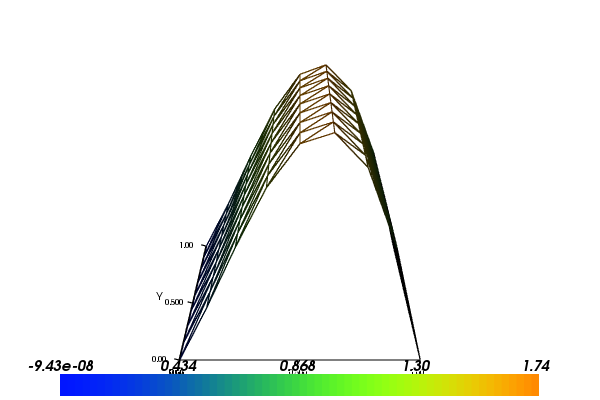
\includegraphics[width=2.3in]{Image/S2DII//P1_u2_8x8.png}  \\
    \caption{u2: Approximate solution, mesh: 8x8, P1, S2DII}\label{fig:fig_P2_u2_8x8}
  \end{minipage}
  \hspace{0.1in}
  \begin{minipage}[t]{0.4 \textwidth}
    \centering
    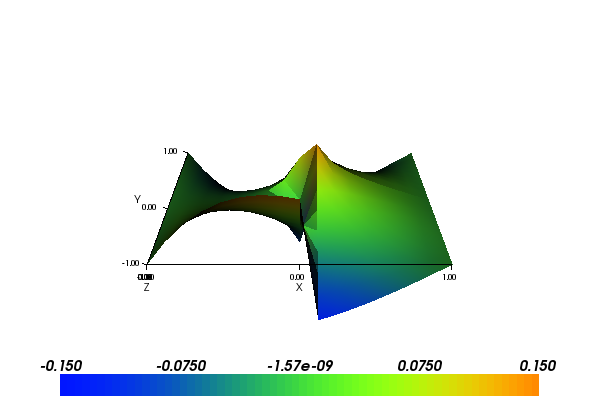
\includegraphics[width=2.3in]{Image/S2DII//P1u2_exact_8x8.png}
    \caption{u2: Exact solution, mesh: 8x8}\label{fig:fig_P2u2_exact_8x8}
  \end{minipage}
\end{figure}

\begin{figure}[bhpt]
  \hspace{35.pt}
  \begin{minipage}[t]{0.4 \textwidth}
    \centering
    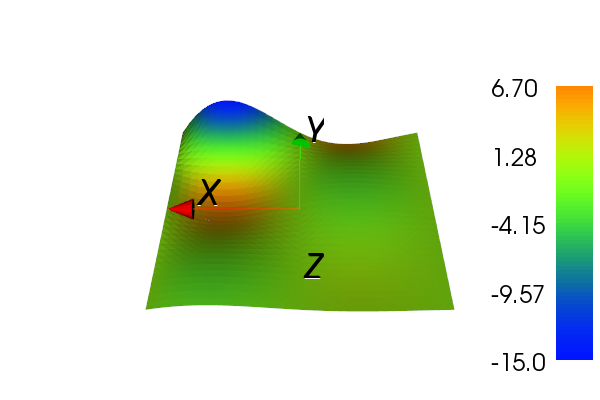
\includegraphics[width=2.3in]{Image/S2DII//P1_u2_16x16.png}\\
    \caption{u2: Approximate solution, mesh: 16x16, P1, , S2DII}\label{fig:fig_P2_u2_16x16}
  \end{minipage}
  \hspace{0.1in}
  \begin{minipage}[t]{0.4 \textwidth}
    \centering
    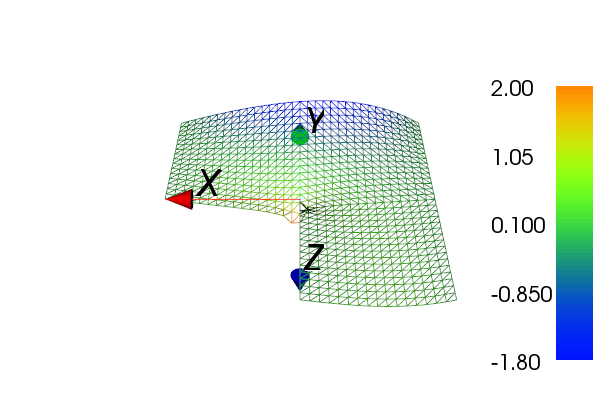
\includegraphics[width=2.3in]{Image/S2DII//P1u2_exact_16x16.png}\\
    \caption{u2: Exact solution, mesh: 16x16}\label{fig:fig_P2u2_exact_16x16}
  \end{minipage}
\end{figure}

\begin{figure}[bhpt]
  \hspace{35.pt}
  \begin{minipage}[t]{0.4 \textwidth}
    \centering
    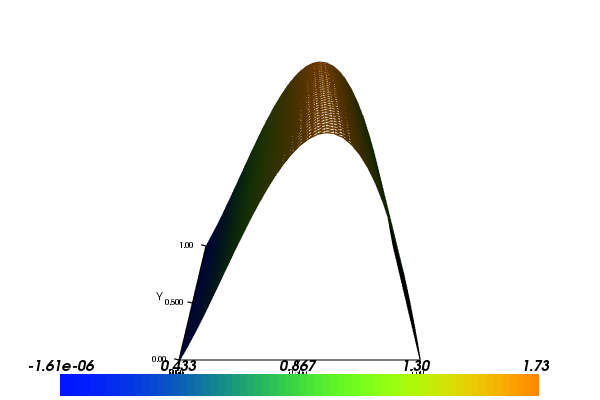
\includegraphics[width=2.3in]{Image/S2DII//P1_u2_32x32.png}\\
    \caption{u2: Approximate solution, mesh: 32x32, P1, S2DII}\label{fig:fig_P2_u2_32x32}
  \end{minipage}
  \hspace{0.1in}
  \begin{minipage}[t]{0.4 \textwidth}
    \centering
    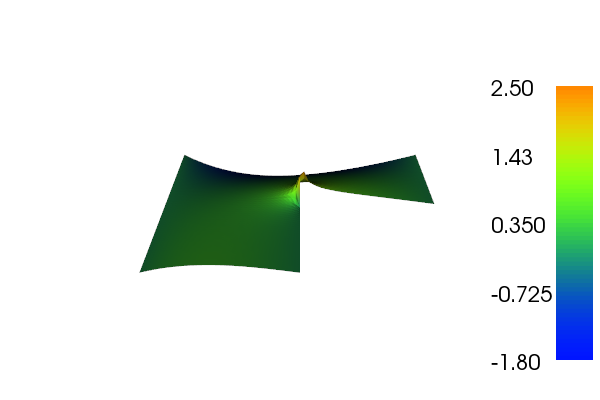
\includegraphics[width=2.3in]{Image/S2DII//P1u2_exact_32x32.png}\\
    \caption{u2: Exact solution, mesh: 32x32}\label{fig:fig_P2u2_exact_32x32}
  \end{minipage}
\end{figure}

\begin{figure}[bhtp]
  \hspace{35.pt}
  \begin{minipage}[t]{0.4 \textwidth}
    \centering
    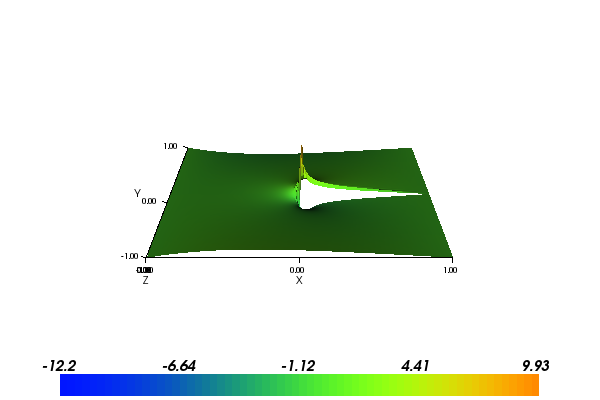
\includegraphics[width=2.3in]{Image/S2DII//P1_u2_64x64.png}\\
    \caption{u2: Approximate solution, mesh: 64x64, P1, S2DII}\label{fig:fig_P2_u2_64x64}
  \end{minipage}
  \hspace{0.1in}
  \begin{minipage}[t]{0.4 \textwidth}
    \centering
    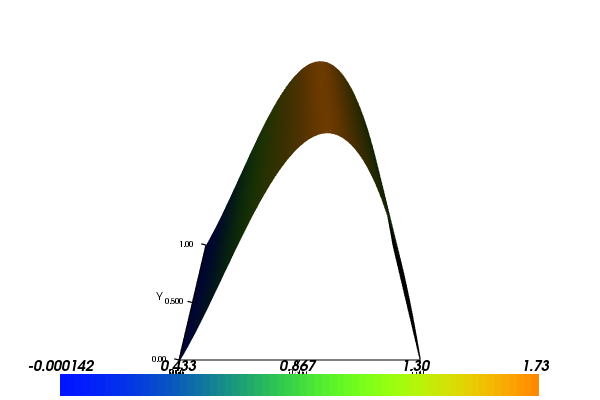
\includegraphics[width=2.3in]{Image/S2DII//P1u2_exact_64x64.png}\\
    \caption{u2: Exact solution, mesh: 64x64}\label{fig:fig_P2u2_exact_64x64}
  \end{minipage}
\end{figure}

\begin{figure}[bhtp]
  \hspace{35.pt}
  \begin{minipage}[t]{0.4 \textwidth}
    \centering
    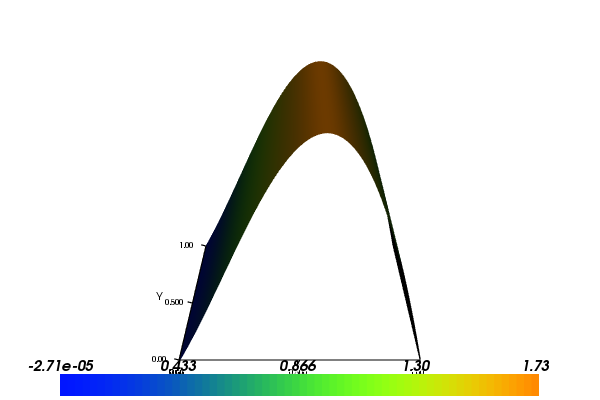
\includegraphics[width=2.3in]{Image/S2DII//P1_u2_128x128.png}\\
    \caption{u2: Approximate solution, mesh: 128x128, P1, S2DII}\label{fig:fig_P2_u2_128x128}
  \end{minipage}
  \hspace{0.1in}
  \begin{minipage}[t]{0.4 \textwidth}
    \centering
    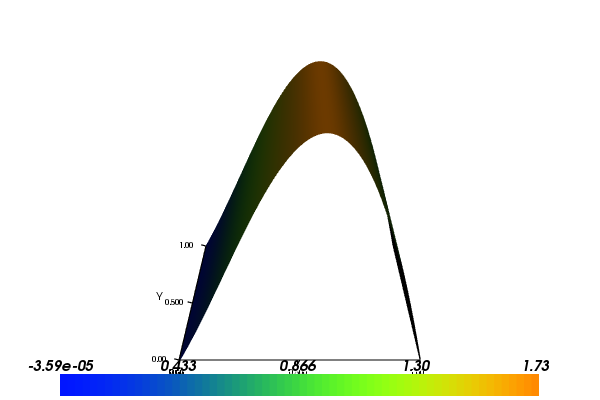
\includegraphics[width=2.3in]{Image/S2DII//P1u2_exact_128x128.png}\\
    \caption{u2: Exact solution, mesh: 128x128}\label{fig:fig_P2u2_exact_128x128}
  \end{minipage}
\end{figure}
\newpage
\begin{figure}[bhtp]
  \hspace{35.pt}
  \begin{minipage}[t]{0.4 \textwidth}
    \centering
    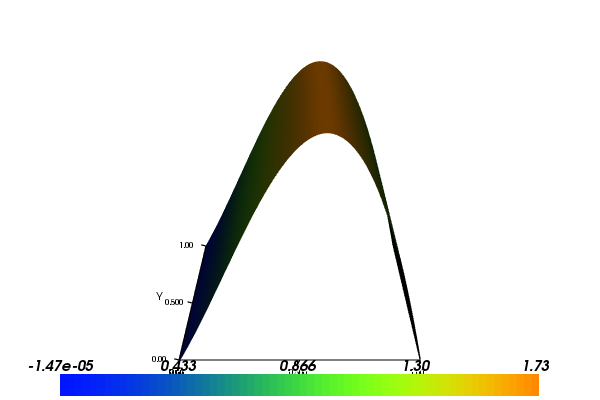
\includegraphics[width=2.3in]{Image/S2DII//P1_u2_256x256.png}\\
    \caption{u2: Approximate solution, mesh: 256x256, P1, S2DII}\label{fig:fig_P2_u2_256x256}
  \end{minipage}
  \hspace{0.1in}
  \begin{minipage}[t]{0.4 \textwidth}
    \centering
    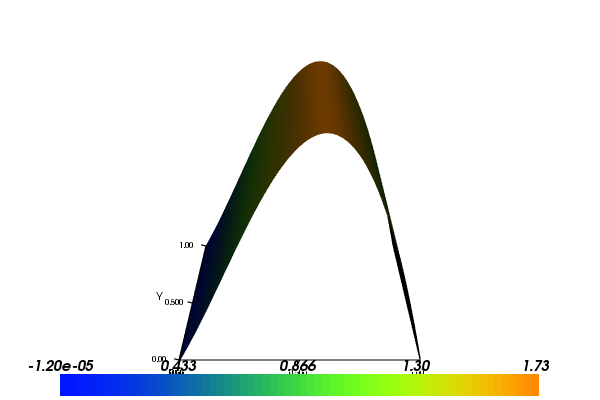
\includegraphics[width=2.3in]{Image/S2DII//P1u2_exact_256x256.png}\\
    \caption{u2: Exact solution, mesh: 256x256}\label{fig:fig_P2u2_exact_256x256}
  \end{minipage}
\end{figure}
N2DII
\begin{figure}[bhtp]
  \hspace{35.pt}
  \begin{minipage}[t]{0.4 \textwidth}
    \centering
    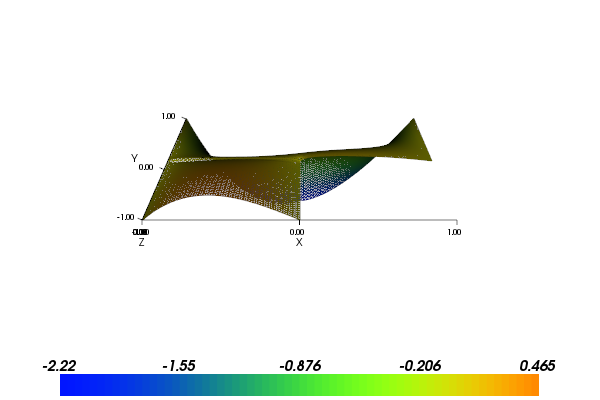
\includegraphics[width=2.3in]{Image/N2DII//P2_u2_32x32.png}\\
    \caption{u2: Approximate solution, mesh: 32x32, P2, N2DII}\label{fig:fig_P2_u2_32-32}
  \end{minipage}
  \hspace{0.1in}
  \begin{minipage}[t]{0.4 \textwidth}
    \centering
    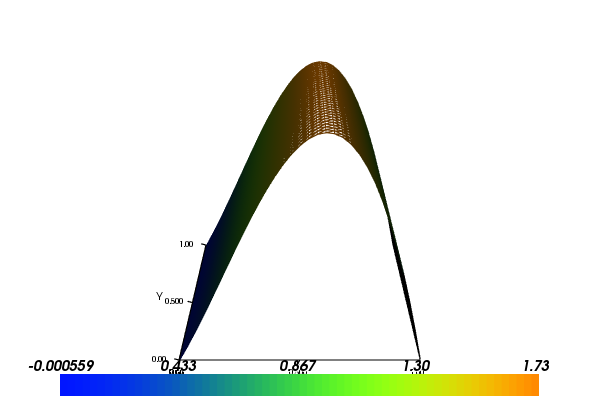
\includegraphics[width=2.3in]{Image/N2DII//P2u2_exact_32x32.png}\\
    \caption{u2: Exact solution, mesh: 32x32}\label{fig:fig_P2u2_exact_32-32}
  \end{minipage}
\end{figure}

\subsection{Conclusion}
\begin{itemize}
  \item S2DI,S2DII has exact error rate.
  \item N2DI,N2DII has not exact error rate while in classical finite element method.
\end{itemize}

\subsection{Do next}
\begin{itemize}
  \item Finite Element Methods: Learning and implementing projection finite element method.
  \item Finite Element Problem: non-smoothing solution, Maxwell eigenproblem.
  \item Finite Element Domain: Cracked square, multi-materials(square for transmission problems), 3D.
\end{itemize}
\end{document}
